
\subsection{Les tâches et techniciens}
Soit $\tech=\{\tech_1,\ldots,\tech_\ntech \}$ un ensemble de $\ntech$ techniciens et $\task=\{\task_1,\ldots,\task_{\ntask}\} $ un ensemble de $\ntask$ tâches que les techniciens peuvent effectuer et $\task = \taskind \cup \taskpred \cup \tasksame \cup \taskapp$ avec $\taskind$ l'ensemble des tâches indépendantes, $\taskpred$ l'ensemble des tâches avec précédence, $\tasksame$ l'ensemble des tâches qui appartiennent à des contraintes de même technicien (Same technician en anglais), $\taskapp$ l'ensemble des tâches qui appartiennent à des contraintes de pré-assignation (Appointments en anglais). On a $\taskind \cap \taskpred = \emptyset$, $\taskind \cap \tasksame = \emptyset$ et $\taskind \cap \taskapp = \emptyset$.

Les techniciens ne travaillent pas en équipe. Donc une tâche ne peut être effectuée que par un seul technicien. Un technicien peut effectuer plusieurs tâches dans la même journée.

On note $p_j$ la durée de la tâche $j$ qui ne dépend pas du technicien. 
Une tâche est définie par une date de  disponibilité ("release date") notée $r_j$, une date de complétion maximale ("due date") notée $d_j$
\footnote{Dans les données clients nous avons des "start due date",notée $sd_j$, (la date à laquelle on doit commencer la tâche avant d'être en retard) et non des "due date" (la date à laquelle on doit terminer la tâche avant d'être en retard). On peut transformer facilement la "start due date" en "due date" : $d_j = sd_j + p_j$.}
, et une date limite ("deadline date") notée $\tilde{d}_j$.


La date de disponibilité est la date à laquelle on peut commencer la tâche au plus tôt. 
La date de complétion maximale est la date à laquelle on doit terminer la tâche au plus tard (si on dépasse cette date, on est en retard).
La date limite est la date après laquelle on ne plus plus effectuer la tâche (plus de retard possible).
On considère $\omega_j$ la priorité de la tâche $j$, $\omega_j$ est calculé en fonction du revenu de la tâche, du retard par rapport à $d_j$ etc.
\subsection{Les fenêtres temporelles}
Les techniciens ont des horaires de travail journaliers qu'ils doivent respecter, on les modélise par un intervalle $[\htech{1}{p},\htech{2}{p}]$ avec $\htech{1}{p}$ pour le début de sa journée et $\htech{2}{p}$ pour la fin de sa journée de travail. De plus, les lieux où les tâches doivent être effectuées ont aussi des horaires d'ouverture qui doivent également être respectés, on le modélise par un intervalle $[\htask{j}{1},\htask{j}{2}]$ avec $\htask{j}{1}$ pour l'heure d'ouverture et $\htask{j}{2}$ pour l'heure de fermeture.
Dans cette intervalle de temps le technicien (resp. la tâche) peut être disponible ou non.

On peut voir les horaires de travail d'un technicien (resp. les horaires d'ouverture d'une tâche) comme étant l'union d'un ensemble d'intervalles où le technicien (resp. la tâche) est disponible et un ensemble d'intervalles où le technicien (resp. la tâche) est indisponible. 

Soit $\overline{\mathcal{K}}^p$ (resp. $\twTech{p}$) l'ensemble des intervalles représentant les périodes d'indisponibilités (resp. disponibilités) du technicien $p$.
Soit $\overline{\mathcal{K}}^j$ (resp. $\twTask{j}$) l'ensemble des intervalles représentant les périodes d'indisponibilités (resp. disponibilités) de la tâche $j$.
Pendant les périodes d'indisponibilités aucune tâche ne peut être commencée ou terminée.

%%%%%%%%%%%%%%%%%%%%%%%%%%%%%%%%%%%%%
\begin{figure}[H]
\centering
\begin{tikzpicture}
   
    \node[scale=4,inner sep=0pt,outer sep=0pt,label=above:Départ] (0) at (0,0) {[};
    \node[scale=4,inner sep=0pt,outer sep=0pt,label=above:Arrivée] (1) at (10,0) {]};
    \node[task={0.2cm}{1cm}{above:activité}] (4) at (2,0){};
\unavailability{5}{4pt}{-4pt}{8}{2}{3}
    
    \draw[] (0.center)--(4.west)node[midway,label=above:trajet]{};
    \draw[] (4.east)--(2)node[midway,label=above:pause]{};
    
    \draw[] (3)--(1.center)node[midway,label=above:trajet]{};
    
    %%%%%%% legende %%%%%%%
 \draw[very thick] (1,-1.15) -- (1,-0.85);
    \draw[very thick] (2.5,-1.15) -- (2.5,-0.85);
 \draw[decorate, decoration=snake] (1,-1)--(2.5,-1)node[pos=1,right]{ = Indisponibilité};
 
 \node[task={0.2cm}{1cm}{right: \text{Une tâche}}] (4) at (1.7,-1.5){};
 %%%%%%%%%%%%%%%%%%
  \end{tikzpicture}
  
\caption{Représentation de la journée de travail d'un technicien.\label{fig:timelineTech}}
\end{figure}
%%%%%%%%%%%%%%%%%%%%%%%%%%%%%%%%%%%%

La figure~\ref{fig:timelineTech} représente une journée possible pour un technicien. Le technicien ne peut pas commencer à se déplacer avant d'avoir commencé sa journée. De plus, il doit être à sa position d'arrivée à la fin de son temps de travail. Le technicien peut être en attente entre la réalisation de deux tâches.


La figure~\ref{fig:badTW} montre un mauvais ordonnancement de tâches  pour un technicien.
Une tâche ne peut pas commencer dans un intervalle de temps où le technicien est indisponible, cf. c).
Une tâche ne peut terminer dans un intervalle de temps où le technicien est indisponible, cf. b). 
Une tâche ne peut pas commencer dans un intervalle de temps d'un technicien et terminer dans un autre intervalle de temps, cf. a). 
Nous avons décidé de modéliser le fait que les techniciens puissent se déplacer pendant les périodes d'indisponibilité.
Cette décision représente un choix lié au problème, on pourrait interdire au technicien de se déplacer vers des tâches pendant leur période d'indisponibilité. 
%%%%%%%%%%%%%%%%%%%%%%%%%%%%%%%%%%%%%%%%%%%%
\begin{figure}[H]
\centering
\begin{tikzpicture}
   
    \node[scale=4,inner sep=0pt,outer sep=0pt,label=above:Départ] (0) at (0,0) {[};
    \node[scale=4,inner sep=0pt,outer sep=0pt,label=above:Arrivée] (1) at (10,0) {]};
    \node[task={0.3cm}{2cm}{above:a)}] (4) at (2.3,0){};
    \node[task={0.3cm}{1.5cm}{above:b)}] (5) at (5,0){};
     \node[task={0.3cm}{1.5cm}{above:c)}] (6) at (8,0){};
\unavailability{5}{2pt}{-2pt}{8}{2}{3}
 \unavailability{2}{2pt}{-2pt}{3}{7}{8}   
    \draw[] (0.center)--(4.west)node[midway,label=above:trajet]{};
    \draw[] (4.east)--(5.west)node[midway,label=above:trajet]{};
    \node at (6.5,0.35) {trajet};
    \draw[] (6.east)--(1.center){};

    %%%%%%% legende %%%%%%%
 \draw[very thick] (1,-1.15) -- (1,-0.85);
    \draw[very thick] (2.5,-1.15) -- (2.5,-0.85);
 \draw[decorate, decoration=snake] (1,-1)--(2.5,-1)node[pos=1,right]{ = Indisponibilité};
 
 \node[task={0.2cm}{1cm}{right: \text{Une tâche}}] (4) at (1.7,-1.5){};
	%%%%%%% legende %%%%%%%
  \end{tikzpicture}
\caption{Problème avec les fenêtres temporelles.\label{fig:badTW}}
\end{figure}
%%%%%%%%%%%%%%%%%%%%%%%%%%%%%%%%%%%%%%%%%%%%


\subsection{La matrice de distances/transitions}
Les techniciens ont un point de départ (là où ils commencent la journée : \textit{startLocation}) et un point d'arrivée (là où ils terminent la journée : \textit{endLocation}).
Pour effectuer une tâche, un technicien doit se déplacer de sa position vers la position associée à la tâche à exécuter, les distances entre les points respectent la distance euclidienne.

 On a donc une matrice $M$ de distance euclidienne de taille au plus $(2\ntech+\ntask)\times(2\ntech+\ntask)$ ($\ntask$ positions pour les tâches et $2\ntech$ positions pour les techniciens : \textit{startLocation} et \textit{endLocation}.
 Un coefficient $m_{ij}$ de la matrice correspond à la distance entre le point $i$ et le point $j$, on suppose que la matrice est symétrique.

On modélise les positions par un graphe orienté pondéré $G=(V,E,M)$ où l'ensemble des sommets $V=V_{depart}\cup V_{arrive}\cup V_{tache}$ représente les points de départ, d'arrivée des techniciens et les positions des tâches. L'ensemble des arêtes E représente le fait de se déplacer d'une position à une autre et $M = (\dist{i}{j})_{(v_i,v_j)\in E}$ représente la matrice de coût des déplacements définie sur $E$.

Par exemple sur la figure~\ref{fig:grapheDist}, un graphe représentant les distances entre cinq sommets, trois sommets (en bleu et plein) pour les positions des tâches et deux sommets pour le point de départ (en rouge et hachuré) et le point d'arrivée (en vert et épais) d'un technicien. Supposons que le technicien débute sa journée (il est donc en position 1) et qu'il doive effectuer la tâche qui est en position 2 alors le coût du déplacement est de 2.

\begin{figure}[H]
\centering
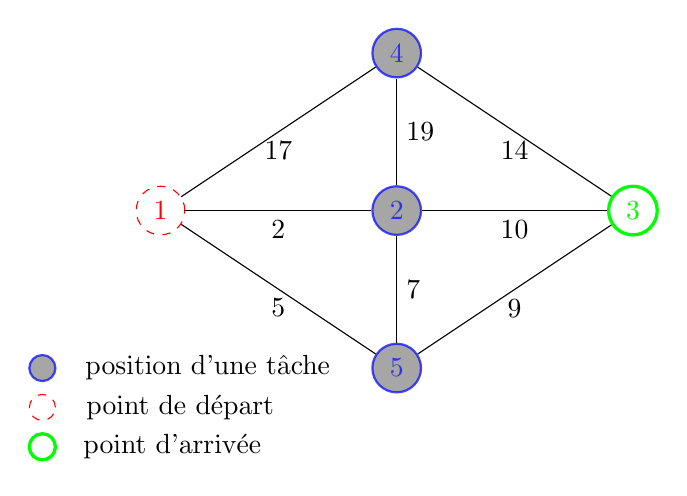
\begin{tikzpicture}

\node[draw,circle,color=red,dashed] (1) at (-3,2) {1};
\node[draw,circle,color=blue,fill=gray,opacity=0.7,thick] (2) at (0,2) {2};
\node[draw,circle,color=green,very thick] (3) at (3,2) {3};
\node[draw,circle,color=blue,fill=gray,opacity=0.7,thick] (4) at (0,4) {4};
\node[draw,circle,color=blue,fill=gray,opacity=0.7,thick] (5) at (0,0) {5};

\node[draw,circle,color=blue,fill=gray,opacity=0.7,thick] (6) at (-4.5,0) {};
\node[] (7) at (-2.4,0) {position d'une tâche};

\node[draw,circle,color=red,dashed] (8) at (-4.5,-0.5) {};
\node[] (9) at (-2.75,-0.5) {point de départ};

\node[draw,circle,color=green,very thick] (10) at (-4.5,-1) {};
\node[] (11) at (-2.85,-1) {point d'arrivée};

\draw (1)--(5) node[midway,below] {$5$};
\draw (1)--(2) node[midway,below] {$2$};
\draw (1)--(4) node[midway,below] {$17$};
\draw (2)--(3) node[midway,below] {$10$};
\draw (5)--(3) node[midway,below] {$9$};
\draw (5)--(2) node[midway,right] {$7$};
\draw (4)--(2) node[midway,right] {$19$};
\draw (4)--(3) node[midway,below] {$14$};
\end{tikzpicture}
\caption{Graphe représentant les distances entre les positions des techniciens et les positions des tâches, ici 1 technicien avec 3 tâches. \label{fig:grapheDist}}
\end{figure}
\par On peut supposer que les techniciens n'admettent pas de contraintes de capacité, ce qui veut dire qu'ils ne doivent pas retourner à un dépôt si leur stock est vide. S'ils ont des contraintes de capacité on peut toujours modéliser cela en insérant le temps de déplacement jusqu'au dépôt dans la durée de la tâche.
\subsection{Les contraintes de précédence}
Pour les tâches trop longues, on autorise la "fragmentation" : la tâche peut être effectuée sur plusieurs jours consécutifs par le même technicien.\\
Soit $\prece \subseteq \taskpred\times \taskpred$ l'ensemble des précédences de tâches :

Soit $(i,j) \in \prece,~ i \not= j :~ C_i~=~t_i + p_i\leq t_j$ avec $t_i$ (resp. $t_j$) la date de début de la tâche $i$ (resp. $j$). Autrement dit, la tâche $i$ doit être terminée avant que la tâche $j$ commence.

\subsection{Les contraintes de compétences}
Les techniciens ont des compétences particulières avec un certain niveau dans chacune d'elle, on peut voir ça comme un vecteur $\alpha^{\tech_i}=(\alpha^{\tech_i}_1,\alpha^{\tech_i}_2,...,\alpha^{\tech_i}_\nskill)$  de $\nskill$ compétences qui prennent des valeurs dans $\{0,..,\nlevel\}$  pour chaque technicien ($0$ veut dire que le technicien ne possède pas la compétence). Les tâches ont des compétences requises, comme pour les techniciens on peut le voir comme un vecteur $\beta^{\task_j}=(\beta^{\task_j}_1,\beta^{\task_j}_2,...,\beta^{\task_j}_\nskill)$ de $\nskill$ compétences qui prennent des valeurs $\{0,...,\nlevel\}$ pour chaque tâche (0 veut dire que la compétence n'est pas requise)\footnote{Les données clients n'arrivent pas sous ce format là, mais on peut facilement les transformer pour qu'elles correspondent à la modélisation.}. Une tâche ne peut pas être effectuée par un technicien qui n'a pas les compétences requises : soit $p\in \tech ~et~ j \in \task,~ \forall i\in[1,..\nskill] ~:~ \gapS{p}{j}{i} \geq 0$.

Par exemple si une tâche $j$ a le vecteur de compétences requises suivant $\beta^j=(0,1,2)$ (la tâche $j$ ne demande aucune compétence dans le domaine "électricien", le niveau 1 de compétence dans le domaine "plombier" et le niveau 2 de compétence dans le domaine "peintre") alors un technicien $p$ qui a les compétences $\alpha^p=(2,1,1)$ ne peut pas réaliser la tâche alors que le technicien $p'$, $\alpha^{p'}=(1,1,2)$, peut l'effectuer.

\section{Les contraintes spécifiques}
Il y a des contraintes spécifiques à notre problème comme les contraintes de même technicien (Same Technician Constraints en anglais, notée \same) ou les contraintes de pré-assignation (Appointements Constraints en anglais, notée \app). 

Les contraintes de même technicien : soit $i,j \in \same$ deux tâches avec une contrainte de même technicien. 
Si un technicien effectue une des deux tâches, alors il sera le seul à pouvoir effectuer la seconde. 
Le technicien peut n'effectuer qu'une seule des deux tâches mais si le technicien n'a pas les compétences pour réaliser une des deux tâches alors il ne peut effectuer aucune des deux tâches.

Il y a trois types de contraintes de pré-assignation : 
\begin{itemize}
\item Pré-assignation d'une tâche à un technicien : soit $j$ une tâche et $p$ un technicien, on associe $j$ à $p$ (cf. figure~\ref{fig:cons:app:time}). Lorsqu'un technicien est pré-assigné à une tâche, ce technicien peut effectuer la tâche même s'il ne possède pas les compétences requises par la tâche.
\item Pré-assignation d'une tâche à un temps : soit $j$ une tâche et $t'_j$ un temps, on fixe $t_{j}=t'_j$ (la date de début de la tâche, cf. figure~\ref{fig:cons:app:time}).
\item Pré-assignation d'une tâche à un technicien et à un temps : soit $j$ une tâche, $p$ un technicien et $t'_{j}$ un temps, on fixe le temps de début de la tâche $t_j=t'_j$ et $p$ le technicien qui l'effectue.
\end{itemize}

Les contraintes de pré-assignation ne sont pas vraiment des contraintes car elles forcent des affectations (i.e. associer une valeur à une variable). Par contre, il reste à savoir si oui ou non la tâche doit être ordonnancée, mais en aucun cas la tâche ne peut être affectée à un autre technicien ou à un autre temps.  




\begin{figure}[H]
\centering
\begin{tikzpicture}
\node[cloud,draw,cloud puffs=10,cloud puff arc=120, aspect=3, inner ysep=1.1em] (0) at (0,0) {$\mathcal{P}$};
\node[] (1) at (5,0) {tâche $j$};

\draw[]  (0.south east)--(1);
\draw[]  (0.north east)--(1) node[midway,above,sloped]{\'{A} quel technicien ?};
\draw[]  (0.east)--(1);

\node[] (2) at (0,-3) {tâche $j$};
\node[] (3) at (5,-3) {technicien $p$};


\draw[]  (2)--(3) node[midway,above]{\'{A} quelle heure ?};

\end{tikzpicture}
\caption{Schéma illustrant la contrainte de pré-assignation d'une tâche à un temps ou à un technicien (ou les deux).\label{fig:cons:app:time}}
\end{figure}


